% ============================================================
%  بخش ۱ — مقدمه
% ============================================================

% ------------------------------------------------------------
\subsection{انگیزه و زمینه‌ی مسئله}
\label{subsec:motivation}
% ------------------------------------------------------------

پروژه‌های زیرساختی و مهندسی بزرگ به\zwnj{}طور مکرر از بودجه و زمان‌بندی
خود تجاوز می\zwnj{}کنند \citep{Flyvbjerg2003, Merrow2011}.
وقتی سبدی از این پروژه‌ها با یک تعهد سرمایه‌ی مشترک به\zwnj{}صورت
هم\zwnj{}زمان اجرا می\zwnj{}شوند، خطرات مضاعف می\zwnj{}شوند:
کوتاهی در عملکرد یک پروژه از طریق بودجه‌ی مشترک به سایرین
سرایت می\zwnj{}کند و تصمیم درباره‌ی میزان تخصیص به هر پروژه
در هر دوره می\zwnj{}تواند سرنوشت موفقیت یا شکست سبد را رقم بزند.

با این حال، پرداختن رسمی به تخصیص بودجه‌ی سطح\zwnj{}سبد به\zwnj{}عنوان
یک مسئله‌ی تصمیم\zwnj{}گیری ترتیبی تا حد زیادی از ادبیات مدیریت
سبد پروژه غایب است.
پژوهش\zwnj{}ها بر مرحله‌ی \emph{انتخاب} تمرکز داشته\zwnj{}اند---
اینکه کدام پروژه\zwnj{}ها گنجانده شوند---
در حالی که مرحله‌ی \emph{حاکمیت عملیاتی}---
چگونگی مدیریت یک سبد متعهدشده تا تکمیل---
توجه تحلیلی نسبتاً کمتری دریافت کرده است
\citep{Archer1999, Cooper2001, Turner2014}.
پژوهش حاضر این شکاف را با ارائه‌ی یک محیط شبیه\zwnj{}سازی تأییدشده
پر می\zwnj{}کند که مسئله را برای روش\zwnj{}های داده\zwnj{}محور قابل حل
می\zwnj{}سازد و یک خط پایه‌ی عملکرد ایجاد می\zwnj{}کند که هزینه‌ی
تخصیص ساده\zwnj{}لوحانه را کمّی می\zwnj{}سازد.

ما سبدی از پروژه\zwnj{}ها را در نظر می\zwnj{}گیریم که هر یک از طریق
یک قرارداد دوطرفه منطبق با فرم‌های \lr{FIDIC} \citep{FIDIC2017}
اداره می\zwnj{}شود و به\zwnj{}صورت هم\zwnj{}زمان زیر یک ذخیره‌ی سرمایه‌ی مشترک
اجرا می\zwnj{}شود.
مدیر سبد در هر دوره‌ی برنامه\zwnj{}ریزی گسسته یک تصمیم تکرارشونده
اتخاذ می\zwnj{}کند: چه مقدار بودجه به هر پروژه‌ی فعال تخصیص دهد.
مسئله‌ی رسمی یافتن سیاست تخصیصی است که جریان نقدی خالص تنزیل\zwnj{}شده
را در سراسر افق سبد بیشینه کند و در عین حال مکانیزم\zwnj{}های قراردادی
را رعایت نماید.

% ------------------------------------------------------------
\subsection{سلسله\zwnj{}مراتب تصمیم\zwnj{}گیری مدیریت پروژه}
\label{subsec:hierarchy}
% ------------------------------------------------------------

سهم حاضر در لایه‌ی حاکمیت سبد از سلسله\zwnj{}مراتب سه\zwnj{}لایه‌ای
مدیریت پروژه عمل می\zwnj{}کند \citep{PMI2017}.
انتخاب سبد---اینکه به کدام پروژه\zwnj{}ها متعهد شود---
به\zwnj{}عنوان یک ورودی برون\zwnj{}زا تلقی می\zwnj{}شود،
منطبق با مدل حاکمیت دومرحله\zwnj{}ای \citet{Turner2014}.
در لایه‌ی حاکمیت، مدیر سبد اجرای پروژه را مستقیماً کنترل نمی\zwnj{}کند
بلکه بودجه را به هر پروژه تخصیص می\zwnj{}دهد و نتایج ارزش کسب\zwnj{}شده
را مشاهده می\zwnj{}کند.
فسخ پروژه یک اقدام عمدی عامل نیست، بلکه یک مکانیزم درون\zwnj{}زای محیط
است که با یکی از دو شرط مستقل فعال می\zwnj{}شود:
یک مهلت سخت که بلافاصله اجرا می\zwnj{}شود اگر دوره‌ی اپیزود به
تاریخ پایان برنامه\zwnj{}ریزی\zwnj{}شده به\zwnj{}علاوه‌ی سقف تأخیر پایان قراردادی برسد؛
یا عملکرد ضعیف پایدار که در آن یک شمارنده‌ی تحمل در هر دوره\zwnj{}ای
که پیشرفت واقعی پروژه از پیشرفت برنامه\zwnj{}ریزی\zwnj{}شده بیشتر از سقف قراردادی
عقب\zwnj{}تر باشد کاهش می\zwnj{}یابد، و فسخ زمانی اجرا می\zwnj{}شود که
شمارنده به صفر برسد.

فسخ پروژه با پایان اپیزود متفاوت است.
یک پروژه به\zwnj{}صورت منفرد فسخ می\zwnj{}شود و یک جریان نقدی تسویه را
فعال می\zwnj{}کند؛ اپیزود تنها زمانی پایان می\zwnj{}یابد که تمام پروژه\zwnj{}ها
یا تکمیل شده یا فسخ شده باشند، افق کلی محقق شده باشد،
یا بودجه‌ی سبد با هیچ ورودی نقدی در راه تمام شده باشد.

\begin{figure}[htbp]
  \centering
  \resizebox{\textwidth}{!}{% figures/feedback_loop.tex
% TikZ only — no figure environment, no caption, no label.
% Include in section file as:
%   % figures/feedback_loop.tex
% TikZ only — no figure environment, no caption, no label.
% Include in section file as:
%   % figures/feedback_loop.tex
% TikZ only — no figure environment, no caption, no label.
% Include in section file as:
%   \input{figures/feedback_loop.tex}
\begin{tikzpicture}[
    every node/.style = {font=\normalsize},
    box/.style = {
      rectangle, rounded corners=6pt,
      draw, thick,
      minimum width=3.4cm, minimum height=1.2cm,
      align=center
    },
    agent/.style  = {box, draw=violet!70!black, fill=violet!10},
    contr/.style  = {box, draw=orange!70!red,   fill=orange!8},
    client/.style = {box, draw=teal!70!black,   fill=teal!8},
    state/.style  = {
      rectangle, rounded corners=6pt,
      draw=gray!60, thick, fill=gray!6,
      minimum width=17cm, minimum height=1.3cm,
      align=center
    },
    act/.style  = {-{Latex[length=6pt]}, thick, violet!70!black},
    rew/.style  = {-{Latex[length=6pt]}, thick, blue!60!black, dashed},
    obs/.style  = {-{Latex[length=6pt]}, thick, gray!50!black},
    prog/.style = {-{Latex[length=6pt]}, thick, orange!70!red},
    int/.style  = {-{Latex[length=6pt]}, thick, teal!60!black, dashed},
    lbl/.style  = {font=\normalsize},
  ]
  
    \node[agent] (pm) {%
      \textbf{Portfolio Manager}\\[2pt]
      policy $\pi(o_t)\!\to\!\boldsymbol{\alpha}_t$};
  
    % --- environment bounding box drawn before interior nodes so it sits behind ---
    % Placeholder client/contractor for fit calculation
    \node[client, right=10cm of pm] (client_ph) {%
      \textbf{Client}\\[2pt]
      milestone approval};
  
    \node[contr, left=3cm of client_ph] (contr_ph) {%
      \textbf{Contractor}\\[2pt]
      project execution};
  
    \node[
      rectangle, rounded corners=20pt,
      draw=orange!50!black, thick, fill=orange!4,
      inner xsep=20pt, inner ysep=18pt,
      fit=(contr_ph)(client_ph),
      label={[font=\footnotesize\itshape, text=orange!60!black]
             above:Environment \textit{(contract)}},
    ] (env) {};
  
    % --- real nodes drawn on top of bounding box ---
    \node[client, right=10cm of pm] (client) {%
      \textbf{Client}\\[2pt]
      milestone approval};
  
    \node[contr, left=3cm of client] (contractor) {%
      \textbf{Contractor}\\[2pt]
      project execution};
  
    % --- observation bar ---
    \node[state,
          below=3.5cm of $(pm.south)!0.55!(contractor.south)$] (obs_bar)
          {\textbf{Observation} $o_t$:\quad
          $\bigl\{\theta^{\mathrm{rem}}_{i,t},\;
          \tilde{x}^{\mathrm{cu}}_{i,t},\;
          \tilde{x}^{\mathrm{cu}+1}_{i,t},\;
          \Delta\psi^*_{i,t},\;
          \widetilde{\Delta\tau}^*_{i,t},\;
          \tilde{x}^*_{i,t},\;
          \widetilde{\mathrm{NPV}}^*_{i,t}\bigr\}_{i=0}^{N-1},\;
          \widetilde{\Delta B}_t,\;
          \tilde{B}_t$};
  
    % --- arrows ---
    \draw[act]
      (pm.east) -- (contractor.west)
      node[midway, above, lbl, violet!80!black]
        {allocation $\boldsymbol{\alpha}_t$};
  
    \draw[prog]
      (contractor.east) -- (client.west)
      node[midway, above, lbl, orange!80!red]
        {progress $\Delta EV_{i,t}$};
  
    \draw[rew]
      (client.north)
        -- ++(0, 1.4)
        -| (pm.north)
      node[pos=0.28, above, lbl, blue!60!black]
        {$r_t = \gamma^{t} \Delta B_t$\quad
         inflow: $\hat{P}_{i,j}$ $+$ $S_i$\quad
         outflow: $x_{i,t}$ $+$ $c^r_{i,t}$};
  
    \draw[prog]
      (contractor.south)
        -- (obs_bar.north -| contractor)
      node[midway, right, lbl]
        {$\Delta EV_{i,t} = \eta_{i,t}\, x_{i,t} / \mathrm{BAC}_i$};
  
    \draw[int]
      (client.east)
        -- ++(1.2, 0)
        |- (obs_bar.east)
      node[pos=0.25, left, lbl, teal!60!black] {milestone revenue};
  
    \draw[obs]
      (obs_bar.west)
        -- ++(-1.2, 0)
        |- (pm.west)
      node[pos=0.25, right, lbl, gray!60!black] {observe $o_t$};
  
  \end{tikzpicture}
\begin{tikzpicture}[
    every node/.style = {font=\normalsize},
    box/.style = {
      rectangle, rounded corners=6pt,
      draw, thick,
      minimum width=3.4cm, minimum height=1.2cm,
      align=center
    },
    agent/.style  = {box, draw=violet!70!black, fill=violet!10},
    contr/.style  = {box, draw=orange!70!red,   fill=orange!8},
    client/.style = {box, draw=teal!70!black,   fill=teal!8},
    state/.style  = {
      rectangle, rounded corners=6pt,
      draw=gray!60, thick, fill=gray!6,
      minimum width=17cm, minimum height=1.3cm,
      align=center
    },
    act/.style  = {-{Latex[length=6pt]}, thick, violet!70!black},
    rew/.style  = {-{Latex[length=6pt]}, thick, blue!60!black, dashed},
    obs/.style  = {-{Latex[length=6pt]}, thick, gray!50!black},
    prog/.style = {-{Latex[length=6pt]}, thick, orange!70!red},
    int/.style  = {-{Latex[length=6pt]}, thick, teal!60!black, dashed},
    lbl/.style  = {font=\normalsize},
  ]
  
    \node[agent] (pm) {%
      \textbf{Portfolio Manager}\\[2pt]
      policy $\pi(o_t)\!\to\!\boldsymbol{\alpha}_t$};
  
    % --- environment bounding box drawn before interior nodes so it sits behind ---
    % Placeholder client/contractor for fit calculation
    \node[client, right=10cm of pm] (client_ph) {%
      \textbf{Client}\\[2pt]
      milestone approval};
  
    \node[contr, left=3cm of client_ph] (contr_ph) {%
      \textbf{Contractor}\\[2pt]
      project execution};
  
    \node[
      rectangle, rounded corners=20pt,
      draw=orange!50!black, thick, fill=orange!4,
      inner xsep=20pt, inner ysep=18pt,
      fit=(contr_ph)(client_ph),
      label={[font=\footnotesize\itshape, text=orange!60!black]
             above:Environment \textit{(contract)}},
    ] (env) {};
  
    % --- real nodes drawn on top of bounding box ---
    \node[client, right=10cm of pm] (client) {%
      \textbf{Client}\\[2pt]
      milestone approval};
  
    \node[contr, left=3cm of client] (contractor) {%
      \textbf{Contractor}\\[2pt]
      project execution};
  
    % --- observation bar ---
    \node[state,
          below=3.5cm of $(pm.south)!0.55!(contractor.south)$] (obs_bar)
          {\textbf{Observation} $o_t$:\quad
          $\bigl\{\theta^{\mathrm{rem}}_{i,t},\;
          \tilde{x}^{\mathrm{cu}}_{i,t},\;
          \tilde{x}^{\mathrm{cu}+1}_{i,t},\;
          \Delta\psi^*_{i,t},\;
          \widetilde{\Delta\tau}^*_{i,t},\;
          \tilde{x}^*_{i,t},\;
          \widetilde{\mathrm{NPV}}^*_{i,t}\bigr\}_{i=0}^{N-1},\;
          \widetilde{\Delta B}_t,\;
          \tilde{B}_t$};
  
    % --- arrows ---
    \draw[act]
      (pm.east) -- (contractor.west)
      node[midway, above, lbl, violet!80!black]
        {allocation $\boldsymbol{\alpha}_t$};
  
    \draw[prog]
      (contractor.east) -- (client.west)
      node[midway, above, lbl, orange!80!red]
        {progress $\Delta EV_{i,t}$};
  
    \draw[rew]
      (client.north)
        -- ++(0, 1.4)
        -| (pm.north)
      node[pos=0.28, above, lbl, blue!60!black]
        {$r_t = \gamma^{t} \Delta B_t$\quad
         inflow: $\hat{P}_{i,j}$ $+$ $S_i$\quad
         outflow: $x_{i,t}$ $+$ $c^r_{i,t}$};
  
    \draw[prog]
      (contractor.south)
        -- (obs_bar.north -| contractor)
      node[midway, right, lbl]
        {$\Delta EV_{i,t} = \eta_{i,t}\, x_{i,t} / \mathrm{BAC}_i$};
  
    \draw[int]
      (client.east)
        -- ++(1.2, 0)
        |- (obs_bar.east)
      node[pos=0.25, left, lbl, teal!60!black] {milestone revenue};
  
    \draw[obs]
      (obs_bar.west)
        -- ++(-1.2, 0)
        |- (pm.west)
      node[pos=0.25, right, lbl, gray!60!black] {observe $o_t$};
  
  \end{tikzpicture}
\begin{tikzpicture}[
    every node/.style = {font=\normalsize},
    box/.style = {
      rectangle, rounded corners=6pt,
      draw, thick,
      minimum width=3.4cm, minimum height=1.2cm,
      align=center
    },
    agent/.style  = {box, draw=violet!70!black, fill=violet!10},
    contr/.style  = {box, draw=orange!70!red,   fill=orange!8},
    client/.style = {box, draw=teal!70!black,   fill=teal!8},
    state/.style  = {
      rectangle, rounded corners=6pt,
      draw=gray!60, thick, fill=gray!6,
      minimum width=17cm, minimum height=1.3cm,
      align=center
    },
    act/.style  = {-{Latex[length=6pt]}, thick, violet!70!black},
    rew/.style  = {-{Latex[length=6pt]}, thick, blue!60!black, dashed},
    obs/.style  = {-{Latex[length=6pt]}, thick, gray!50!black},
    prog/.style = {-{Latex[length=6pt]}, thick, orange!70!red},
    int/.style  = {-{Latex[length=6pt]}, thick, teal!60!black, dashed},
    lbl/.style  = {font=\normalsize},
  ]
  
    \node[agent] (pm) {%
      \textbf{Portfolio Manager}\\[2pt]
      policy $\pi(o_t)\!\to\!\boldsymbol{\alpha}_t$};
  
    % --- environment bounding box drawn before interior nodes so it sits behind ---
    % Placeholder client/contractor for fit calculation
    \node[client, right=10cm of pm] (client_ph) {%
      \textbf{Client}\\[2pt]
      milestone approval};
  
    \node[contr, left=3cm of client_ph] (contr_ph) {%
      \textbf{Contractor}\\[2pt]
      project execution};
  
    \node[
      rectangle, rounded corners=20pt,
      draw=orange!50!black, thick, fill=orange!4,
      inner xsep=20pt, inner ysep=18pt,
      fit=(contr_ph)(client_ph),
      label={[font=\footnotesize\itshape, text=orange!60!black]
             above:Environment \textit{(contract)}},
    ] (env) {};
  
    % --- real nodes drawn on top of bounding box ---
    \node[client, right=10cm of pm] (client) {%
      \textbf{Client}\\[2pt]
      milestone approval};
  
    \node[contr, left=3cm of client] (contractor) {%
      \textbf{Contractor}\\[2pt]
      project execution};
  
    % --- observation bar ---
    \node[state,
          below=3.5cm of $(pm.south)!0.55!(contractor.south)$] (obs_bar)
          {\textbf{Observation} $o_t$:\quad
          $\bigl\{\theta^{\mathrm{rem}}_{i,t},\;
          \tilde{x}^{\mathrm{cu}}_{i,t},\;
          \tilde{x}^{\mathrm{cu}+1}_{i,t},\;
          \Delta\psi^*_{i,t},\;
          \widetilde{\Delta\tau}^*_{i,t},\;
          \tilde{x}^*_{i,t},\;
          \widetilde{\mathrm{NPV}}^*_{i,t}\bigr\}_{i=0}^{N-1},\;
          \widetilde{\Delta B}_t,\;
          \tilde{B}_t$};
  
    % --- arrows ---
    \draw[act]
      (pm.east) -- (contractor.west)
      node[midway, above, lbl, violet!80!black]
        {allocation $\boldsymbol{\alpha}_t$};
  
    \draw[prog]
      (contractor.east) -- (client.west)
      node[midway, above, lbl, orange!80!red]
        {progress $\Delta EV_{i,t}$};
  
    \draw[rew]
      (client.north)
        -- ++(0, 1.4)
        -| (pm.north)
      node[pos=0.28, above, lbl, blue!60!black]
        {$r_t = \gamma^{t} \Delta B_t$\quad
         inflow: $\hat{P}_{i,j}$ $+$ $S_i$\quad
         outflow: $x_{i,t}$ $+$ $c^r_{i,t}$};
  
    \draw[prog]
      (contractor.south)
        -- (obs_bar.north -| contractor)
      node[midway, right, lbl]
        {$\Delta EV_{i,t} = \eta_{i,t}\, x_{i,t} / \mathrm{BAC}_i$};
  
    \draw[int]
      (client.east)
        -- ++(1.2, 0)
        |- (obs_bar.east)
      node[pos=0.25, left, lbl, teal!60!black] {milestone revenue};
  
    \draw[obs]
      (obs_bar.west)
        -- ++(-1.2, 0)
        |- (pm.west)
      node[pos=0.25, right, lbl, gray!60!black] {observe $o_t$};
  
  \end{tikzpicture}}
  \caption{حاکمیت سبد به\zwnj{}صورت یک حلقه‌ی بازخورد یادگیری تقویتی.
    مدیر سبد کسرهای تخصیصی $\boldsymbol{\alpha}_t$ را متعهد می\zwnj{}شود؛
    پیمانکار بودجه را از طریق بازده تصادفی $\eta_{i,t}$ به پیشرفت
    تبدیل می\zwnj{}کند؛ کارفرما نقاط عطف را تأیید کرده و پرداخت\zwnj{}های
    خالص $\hat{P}_{i,j}$ را آزاد می\zwnj{}کند؛
    محیط مشاهده‌ی $o_t \in \mathbb{R}^{7N+2}$ و پاداش $r_t$
    را برمی\zwnj{}گرداند.
    اجزای بردار مشاهده به\zwnj{}طور کامل در جدول~\ref{tab:obs_vector}
    تعریف شده\zwnj{}اند.}
  \label{fig:feedback_loop}
\end{figure}

% ------------------------------------------------------------
\subsection{مکانیزم\zwnj{}های قراردادی و ساختار جریان نقدی}
\label{subsec:contract_mechanics}
% ------------------------------------------------------------

تعامل مالی بین مدیر سبد و هر پیمانکار از طریق فرم\zwnj{}های قراردادی
\lr{FIDIC} \citep{FIDIC2017} اداره می\zwnj{}شود.
سه مکانیزم ساختار جریان نقدی را تعیین می\zwnj{}کنند.

\paragraph{پرداخت مبتنی بر نقطه‌ی عطف.}
پرداخت مشروط به آستانه\zwnj{}های پیشرفت تأییدشده است.
پرداخت ناخالص در نقطه‌ی عطف $j$ کسر ثابتی از
قرارداد قراردادی است.
از آنجا که پرداخت مشروط به پیشرفت تأییدشده است،
زمان\zwnj{}بندی ورودی\zwnj{}های نقدی به عملکرد واقعی پیمانکار و
تصمیمات تخصیص مدیر سبد بستگی دارد.
عدم\zwnj{}قطعیت جریان نقدی در مدل حاضر از یک منبع واحد ناشی می\zwnj{}شود:
بازده تصادفی بودجه\zwnj{}به\zwnj{}پیشرفت $\eta_{i,t}$،
که حاکم است بر اینکه یک تخصیص بودجه‌ی معین در هر دوره
چه مقدار پیشرفت فیزیکی ایجاد می\zwnj{}کند.
بهره\zwnj{}وری نامطمئن منجر به زمان\zwnj{}بندی نقطه‌ی عطف نامطمئن می\zwnj{}شود
که به نوبه‌ی خود منجر به ورود نقدی نامطمئن می\zwnj{}شود---
بدون نیاز به هیچ مدل جداگانه\zwnj{}ای از تأخیر پرداخت.

\paragraph{پیش\zwnj{}پرداخت و بازیابی تدریجی.}
در آغاز پروژه، پیش\zwnj{}پرداختی معادل کسر ثابتی از قیمت قرارداد
به پیمانکار پرداخت می\zwnj{}شود.
این پیش\zwnj{}پرداخت از طریق کسورات درصدی از گواهی\zwnj{}های پرداخت
بین\zwnj{}دوره\zwnj{}ای بعدی بازیابی می\zwnj{}شود،
با آستانه‌ی شروع و نرخ کسر مشخص\zwnj{}شده به\zwnj{}عنوان
پارامترهای قراردادی خاص پروژه \citep{FIDIC2017}.

\paragraph{حسن انجام کار.}
کسری از هر پرداخت نقطه‌ی عطف به\zwnj{}عنوان وثیقه‌ی عملکرد
نگه\zwnj{}داشته می\zwnj{}شود و با تکمیل پروژه به\zwnj{}طور کامل آزاد می\zwnj{}شود،
و یک انگیزه‌ی ساختاری تکمیل را در مکانیزم\zwnj{}های پرداخت جاسازی می\zwnj{}کند.

\paragraph{مدیریت ارزش کسب\zwnj{}شده به\zwnj{}عنوان سیگنال عملکردی.}
چارچوب \lr{EVM} \citep{Fleming2010} واژگان تشخیصی برای
پایش عملکرد پیمانکار را فراهم می\zwnj{}کند.
شاخص عملکرد هزینه و شاخص عملکرد زمان‌بندی ارزش کسب\zwnj{}شده به\zwnj{}ترتیب
کارایی هزینه و کارایی زمان\zwnj{}بندی را اندازه\zwnj{}گیری می\zwnj{}کنند؛
برآورد در تکمیل از یک مخرج مرکب هزینه\zwnj{}و\zwnj{}زمان\zwnj{}بندی
برای پیش\zwnj{}بینی کل مخارج استفاده می\zwnj{}کند؛
و شاخص عملکرد تا تکمیل کارایی مورد نیاز در کار باقی\zwnj{}مانده
برای پایان یافتن در بودجه را اندازه\zwnj{}گیری می\zwnj{}کند.
این چهار شاخص به\zwnj{}صورت داخلی ردیابی شده و در هر دوره
به رکورد حسابرسی ثبت می\zwnj{}شوند، اما مستقیماً در بردار مشاهده
نشان داده نمی\zwnj{}شوند؛ آن\zwnj{}ها به\zwnj{}عنوان میانجی\zwnj{}هایی عمل می\zwnj{}کنند
که از آن\zwnj{}ها ویژگی\zwnj{}های تخصیص جبرانی و نقطه‌ی عطف هدف
مشتق می\zwnj{}شوند.

\paragraph{فسخ قرارداد.}
یک ویژگی متمایز محیط پیشنهادی این است که فسخ پروژه
به\zwnj{}عنوان پیامد درون\zwnj{}زای تصمیمات تأمین مالی خود مدیر
تلقی می\zwnj{}شود، نه یک شوک برون\zwnj{}زا.
در عمل، یک پیمانکار می\zwnj{}تواند یک پروژه را به دو روش کیفاً متفاوت
از دست بدهد: به\zwnj{}تدریج، وقتی کم\zwnj{}تأمینی پایدار اجازه می\zwnj{}دهد
لغزش زمان\zwnj{}بندی از آستانه‌ی تحمل قراردادی فراتر رود
و از یک دوره‌ی مهلتی بگذرد که برای بازیابی در نظر گرفته شده است؛
یا ناگهانی، هنگامی که تاریخ پایان پروژه از حد مجاز قراردادی
تجاوز می\zwnj{}کند صرف\zwnj{}نظر از اینکه تا چه حد به جبران نزدیک است.
تنها گرفتن یکی از این حالت\zwnj{}های شکست---
چنانکه صورت\zwnj{}بندی\zwnj{}های تک\zwnj{}پروژه‌ای قبلی معمولاً انجام می\zwnj{}دهند---
قرارگیری مدیر در معرض ریسک واقعی را دست\zwnj{}کم می\zwnj{}گیرد.
فسخ همچنین پیامدهای مالی مستقیمی دارد که باید
در برابر موضع نقدی سبد تسویه شوند،
زیرا کاری که برایش پرداخت شده و کاری که انجام شده
به ندرت دقیقاً در لحظه‌ی فسخ قرارداد منطبقند.
با جاسازی هر دو شرط نقض، مکانیزم مهلت مرتبط با آن\zwnj{}ها،
و جریان نقدی تسویه‌ی ناشی از آن مستقیماً در دینامیک گذار،
محیط هر سیاستی را مجبور می\zwnj{}کند تهدید فسخ را
به\zwnj{}عنوان پیامد انتخاب\zwnj{}های تخصیصی خودش تلقی کند---
دقیقاً همان ساختار انگیزشی که یک مدیر سبد واقعی با آن روبه\zwnj{}رو است.

% ------------------------------------------------------------
\subsection{شکاف بهینگی و ضرورت سیاست\zwnj{}های یادگیری\zwnj{}شده}
\label{subsec:gap}
% ------------------------------------------------------------

یک سؤال تجربی محوری این است که آیا مسئله به اندازه‌ی کافی دشوار است
که سیاست\zwnj{}های یادگیری\zwnj{}شده را موجه کند.
برای پاسخ به این سؤال، سه اکتشافی قطعی حریصانه را
در برابر یک بهینه‌ی اطلاعات\zwnj{}کامل محاسبه\zwnj{}شده‌ی دستی
روی چهار پیکربندی معیار سبد با پیچیدگی فزاینده اجرا می\zwnj{}کنیم.

اکتشافی \textbf{رسیدن\zwnj{}به\zwnj{}برنامه} ($\pi^{\mathrm{rp}}$) دقیقاً
بودجه‌ی کافی برای رساندن هر پروژه‌ی فعال به پیشرفت برنامه\zwnj{}ریزی\zwnj{}شده‌ی
منحنی\lr{-S} را در هر دوره تخصیص می\zwnj{}دهد و شکاف پیشرفت را
به\zwnj{}طور کامل می\zwnj{}بندد.
اکتشافی \textbf{جبران\zwnj{}-T} ($\pi^{\mathrm{cu}}$) فقط به اندازه‌ای
تخصیص می\zwnj{}دهد که در تحمل تأخیر پیشرفت قراردادی بماند
و مخارج را به حداقل می\zwnj{}رساند.
اکتشافی \textbf{جبران\zwnj{}-T بعدی} ($\pi^{\mathrm{cu}+1}$) محتاط\zwnj{}تر است:
از این دوره به اندازه‌ی کافی پیش\zwnj{}دستانه تخصیص می\zwnj{}دهد
تا تأخیر پیش\zwnj{}بینی\zwnj{}شده در دوره‌ی بعد نیز در محدوده‌ی تحمل بماند.
\textbf{بهینه‌ی اطلاعات\zwnj{}کامل} ($\pi^*$) با تمام تحقق\zwnj{}های تصادفی
از پیش\zwnj{}شناخته\zwnj{}شده به\zwnj{}صورت دستی محاسبه می\zwnj{}شود
و به\zwnj{}عنوان مرجع کران بالا عمل می\zwnj{}کند.

شکل~\ref{fig:gap_plot} \lr{NPV} تجمعی اپیزود را برای هر روش
در چهار پیکربندی گزارش می\zwnj{}دهد.
در ساده\zwnj{}ترین پیکربندی (پروژه‌ی منفرد، بازده ثابت)
خطوط پایه‌ی حریصانه با فاصله‌ی کوچکی به بهینه نزدیک می\zwnj{}شوند.
با افزایش پیچیدگی سبد---پروژه\zwnj{}های بیشتر، شروع\zwnj{}های پلکانی،
جریان\zwnj{}های نقدی متعامل، و قیود توالی نقطه‌ی عطف---
شکاف به\zwnj{}صورت سیستماتیک افزایش می\zwnj{}یابد.
در پیچیده\zwnj{}ترین پیکربندی بهترین خط پایه‌ی حریصانه
بیش از ۶۰ واحد \lr{NPV} از بهینه عقب می\zwnj{}ماند
در حالی که یک خط پایه به نتیجه‌ی زیان\zwnj{}ده تنزل می\zwnj{}کند.
این گسترش یکنواخت تأیید می\zwnj{}کند که مسئله‌ی تخصیص
در مقیاس واقعاً دشوار می\zwnj{}شود و یک هدف بهبود مشخص
برای عامل\zwnj{}های یادگیری تقویتی وجود دارد.

\begin{figure}[H]
    \centering
    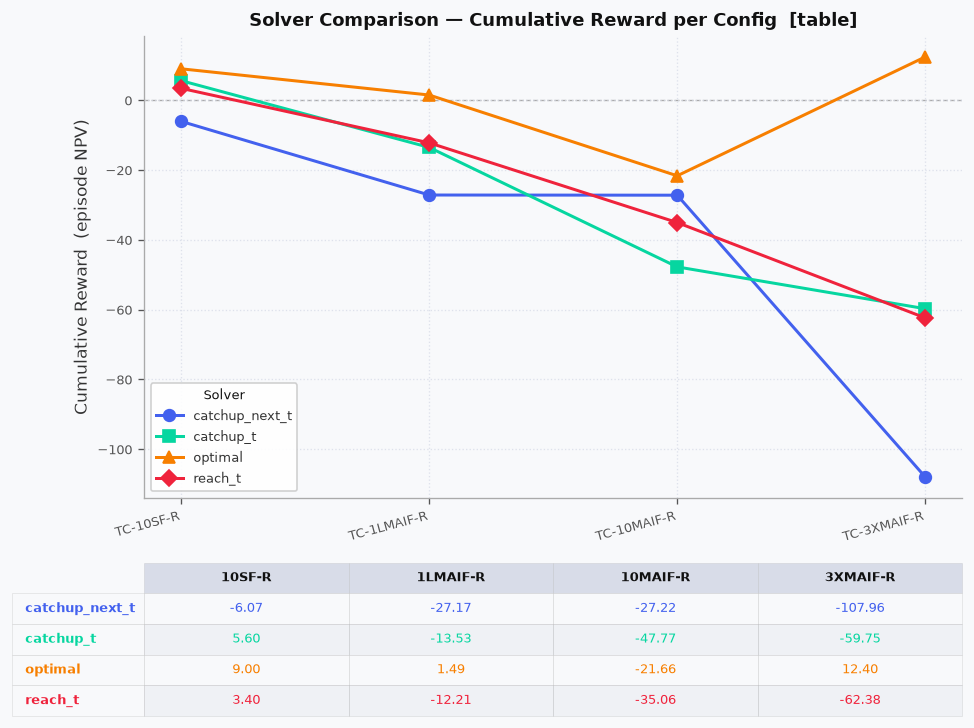
\includegraphics[width=\textwidth]{figures/gap_plot.png}
    \caption{\lr{NPV} تجمعی اپیزود (پاداش) برای سه اکتشافی حریصانه
    و بهینه‌ی اطلاعات\zwnj{}کامل در چهار پیکربندی معیار با پیچیدگی
    سبد فزاینده. شکاف رو به افزایش با رشد پیچیدگی
    استفاده از سیاست\zwnj{}های تخصیصی یادگیری\zwnj{}شده را توجیه می\zwnj{}کند.}
    \label{fig:gap_plot}
\end{figure}

% ------------------------------------------------------------
\subsection{مشارکت\zwnj{}ها و ساختار مقاله}
\label{subsec:organisation}
% ------------------------------------------------------------

مشارکت\zwnj{}های این مقاله سه\zwnj{}گانه است.

\begin{enumerate}[leftmargin=*, label=\textbf{م\arabic*.}]

    \item \textbf{محیط.}
    یک محیط \lr{MDP} پیکربندی\zwnj{}پذیر سازگار با \lr{Gymnasium}
    که چرخه‌ی کامل جریان نقدی قرارداد \lr{FIDIC} را رمزگذاری می\zwnj{}کند:
    پیش\zwnj{}پرداخت و بازیابی تدریجی، پرداخت\zwnj{}های نقطه‌ی عطف
    وزن\zwnj{}دهی\zwnj{}شده با پیشرفت، کسر و آزادسازی حسن انجام کار،
    بهره‌ی برداشت از خزانه بر موجودی\zwnj{}های نقدی منفی پروژه،
    و یک دروازه‌ی فسخ دوشرطی با یک شمارنده‌ی دوره‌ی مهلت
    خاص پروژه.
    تمام پارامترهای محیط از طریق یک دیکشنری پیکربندی
    مشخص می\zwnj{}شوند که مدخل\zwnj{}هایش توزیع\zwnj{}های احتمال هستند
    و به پیشه\zwnj{}ورزان در هر بخش مبتنی بر پروژه---
    ساخت\zwnj{}وساز، فناوری اطلاعات، تحقیق\zwnj{}و\zwnj{}توسعه، یا غیره---
    اجازه می\zwnj{}دهد با برازش آن توزیع\zwnj{}ها بر داده\zwnj{}های تاریخی شرکت،
    محیط\zwnj{}های خاص حوزه را نمونه\zwnj{}سازی کنند.
    انطباق با \lr{API} گیمنازیوم در ۵۱ بررسی در ۱۰ بخش آزمون
    تأیید شده است؛ گواهی سازگاری کامل در پیوست~\ref{app:gym_certificate}
    بازتولید شده است.
    محیط با یک دفتر کل حسابرسی \lr{SQLite} ارائه می\zwnj{}شود که
    هر تخصیص، رویداد جریان نقدی، و پرچم نقض را در هر گام اپیزود
    ثبت می\zwnj{}کند و رفتار سیاست را کاملاً قابل تفسیر می\zwnj{}سازد.

    \item \textbf{صورت\zwnj{}بندی \lr{MDP}.}
    یک مشخصات رسمی از مسئله‌ی بودجه\zwnj{}بندی سبد به\zwnj{}عنوان یک
    فرایند تصمیم\zwnj{}گیری مارکوف: فضای حالت، فضای عمل،
    دینامیک گذار، سیگنال پاداش، و بردار مشاهده
    در قالب بسته، با همسویی کامل میان مشخصات ریاضی
    و محیط پیاده\zwnj{}سازی\zwnj{}شده.

    \item \textbf{معیار خط پایه و شکاف بهینگی.}
    سه اکتشافی قطعی حریصانه ارزیابی\zwnj{}شده در برابر یک بهینه‌ی
    اطلاعات\zwnj{}کامل در چهار پیکربندی معیار،
    که یک شکاف بهینگی کمّی‌شده ایجاد می\zwnj{}کند که به\zwnj{}صورت یکنواخت
    با پیچیدگی سبد رشد می\zwnj{}کند و هدف عملکردی را برای
    عامل\zwnj{}های یادگیری تقویتی آینده تعیین می\zwnj{}کند.

\end{enumerate}

بخش~\ref{sec:literature} ادبیات مرتبط را در چهار جریان مرور می\zwnj{}کند:
مبانی مدیریت پروژه، مدیریت و انتخاب سبد،
بودجه\zwnj{}بندی \lr{PPM} و مدل\zwnj{}سازی جریان نقدی،
و یادگیری تقویتی برای تخصیص منابع ترتیبی.
بخش~\ref{sec:problem} صورت\zwnj{}بندی \lr{MDP} را به\zwnj{}صورت رسمی
توسعه می\zwnj{}دهد.
بخش~\ref{sec:evaluation} ارزیابی معیار را ارائه می\zwnj{}دهد:
سه اکتشافی قطعی حریصانه و یک بهینه‌ی اطلاعات\zwnj{}کامل
در چهار پیکربندی سبد، که شکاف بهینگی انگیزه\zwnj{}بخش
عامل\zwnj{}های یادگیری\zwnj{}شده را کمّی می\zwnj{}سازد.
آموزش عامل\zwnj{}های \lr{RL} روی محیط به\zwnj{}عنوان گام طبیعی بعدی
باقی می\zwnj{}ماند که در کارهای بعدی به آن پرداخته می\zwnj{}شود.